%-------------------------------------------------------------------------------------------------------
%-------------------------------------------------------------------------------------------------------
% Sec & Label

\section{Introduction}
\label{sec:introduction}

%-------------------------------------------------------------------------------------------------------
%-------------------------------------------------------------------------------------------------------


The objective of this laboratory assignment is to create a BandPass Filter (BPF) circuit using one OP-AMP with a gain at central frequency of 40db and a central frequency of 1000Hz. The goal is then to attain the maximum value for the Merit (M) by modifying the circuit and its components with some restricted. The expression for M is as follows:

\[
M = \frac{1}{Cost\times (CentralfFreqDev + GainDev + 10^{-6})}
\]

\[
 Cost = Cost_{resistors} + Cost_{capacitors} + Cost_{transistors} + Cost_{diodes} 
\] \\

$Cost_{resistors} = 1MU/kOhm$; $Cost_{capacitors} = 1MU/\mu F$; $Cost_{diodes} = 0.1MU/diode$; $Cost_{transistors} = 0.1MU/transistor$ \\

The final circuit, displayed in figure \ref{fig:Desenho_t4}, utilizes the following components:

\begin{itemize}
	\item three voltage sources ($V_{in}$ - sinusoidal, $V_{cc}$ and $V_{ee}$)
	\item one 741 OP-AMP
	\item three resistors ($R_1$, $R_2$ and $R_3$)
	\item one capacitors ($C_1$)
\end{itemize}

The values associated with each component is displayed on Table \ref{tab:vlr}. The OP-AMP used was already provided as well as the voltage source $V_{in}$.

\begin{table}[ht]
	\centering
	\begin{tabular}{|l|r|}
		\hline    
		{\bf Name} & {\bf Value} \\ \hline
    		
$V_{cc}$	&	5.00	\\ \hline
$V_{ee}$	&	-5.00	\\ \hline

$R1$	&	1.0k	\\ \hline
$R2$	&	100.0k	\\ \hline
$R3$	&	10.0k	\\ \hline
$C_1$	&	220.0n	\\ \hline



	\end{tabular}
	
	\caption{Components' values.}
    
\label{tab:vlr}
\end{table}


\begin{figure}[ht]
	\centering
	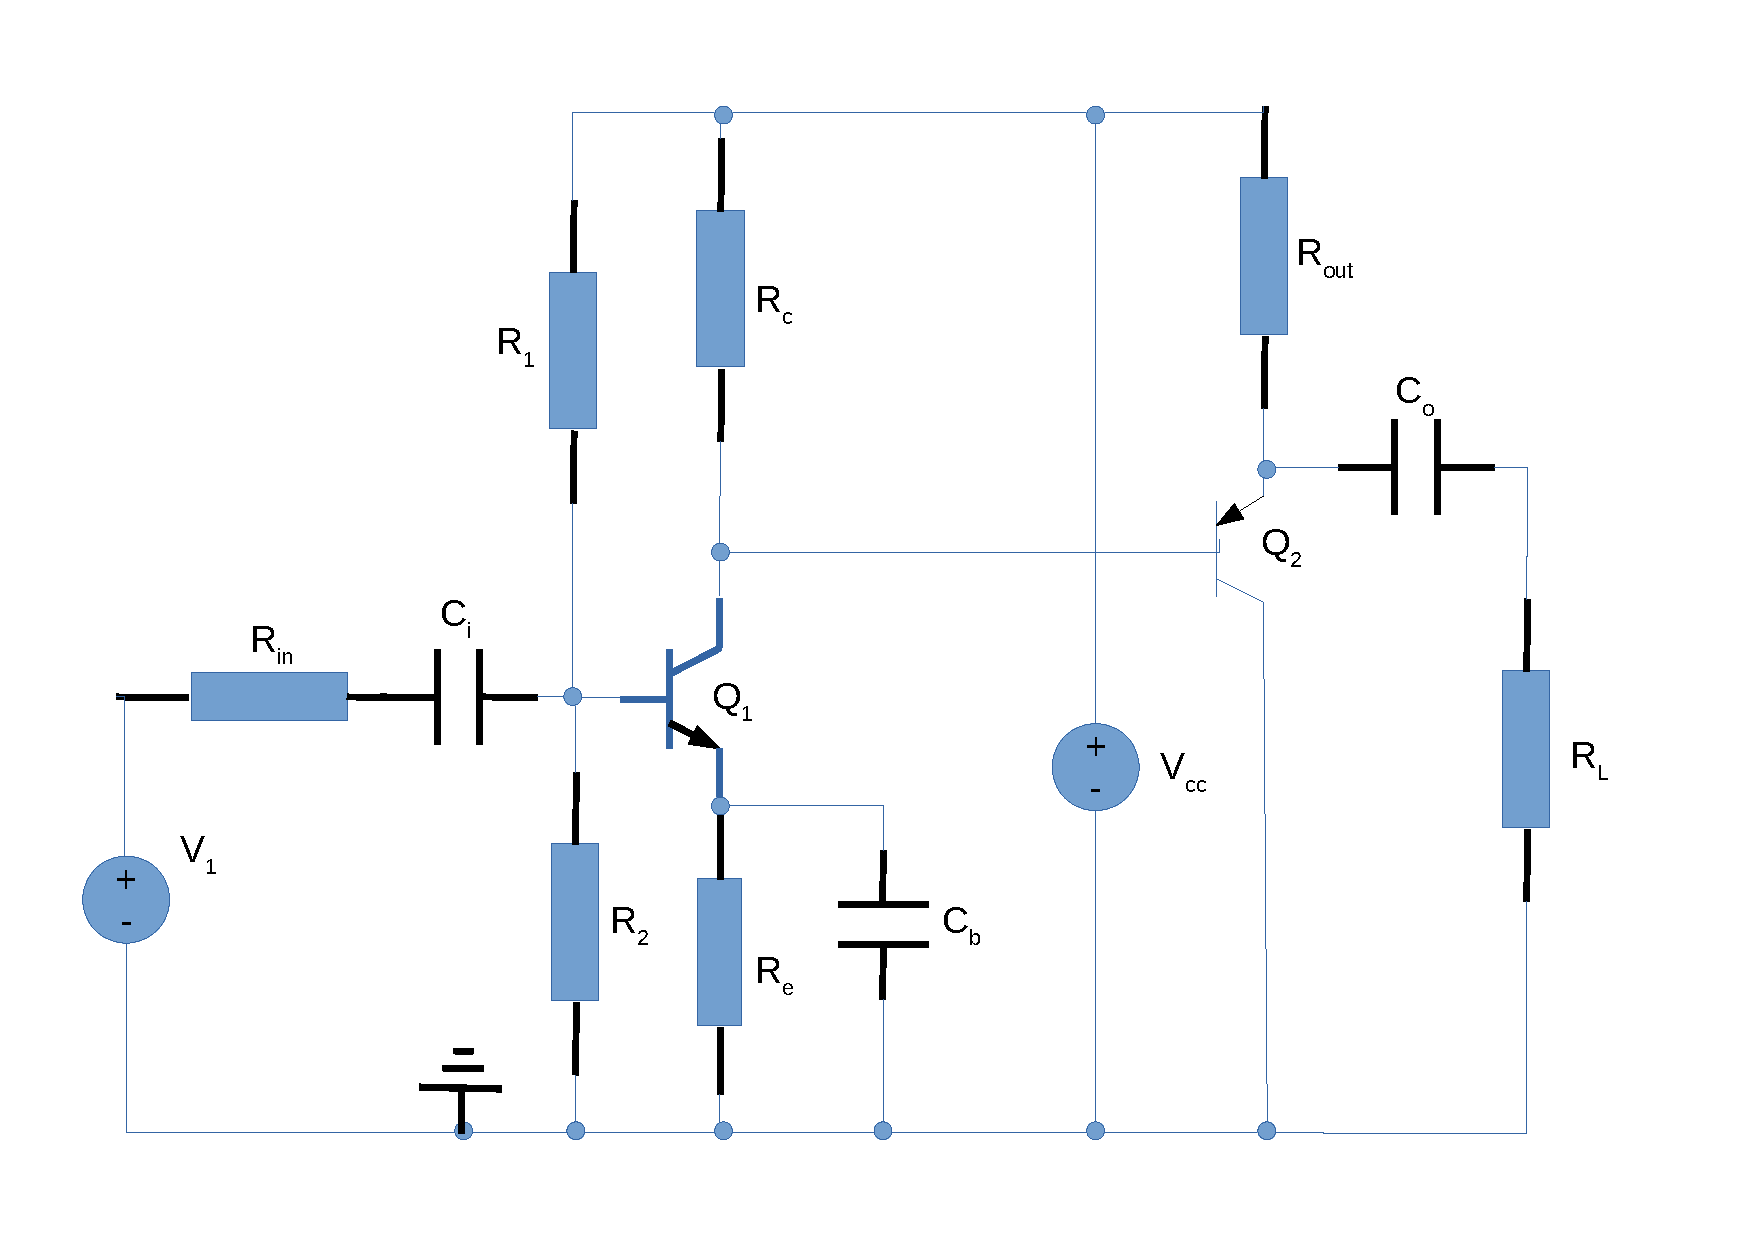
\includegraphics[width=0.85\linewidth]{dsnh_t4.pdf}
	\caption{Circuit T4}
\label{fig:Desenho_t4}
\end{figure}

Theoretical and simulation analysis are presented in Section \ref{sec:analysis} and Section \ref{sec:simulation}, respectively, and the results of each are then compared.
Finally, in Section \ref{sec:conclusion} the conclusions of the laboratory assignment are outlined.

